% This is sigproc-sp.tex -FILE FOR V2.6SP OF ACM_PROC_ARTICLE-SP.CLS
% OCTOBER 2002
%
% It is an example file showing how to use the 'acm_proc_article-sp.cls' V2.6SP
% LaTeX2e document class file for Conference Proceedings submissions.
% ----------------------------------------------------------------------------------------------------------------
% This .tex file (and associated .cls V2.6SP) *DOES NOT* produce:
%       1) The Permission Statement
%       2) The Conference (location) Info information
%       3) The Copyright Line with ACM data
%       4) Page numbering
%
%  However, both the CopyrightYear (default to 2002) and the ACM Copyright Data
% (default to X-XXXXX-XX-X/XX/XX) can still be over-ridden by whatever the author
% inserts into the source .tex file.
% e.g.
% \CopyrightYear{2003} will cause 2003 to appear in the copyright line.
% \crdata{0-12345-67-8/90/12} will cause 0-12345-67-8/90/12 to appear in the copyright line.
%
% ---------------------------------------------------------------------------------------------------------------
% It is an example which *does* use the .bib file (from which the .bbl file
% is produced).
% REMEMBER HOWEVER: After having produced the .bbl file,
% and prior to final submission,
% you need to 'insert'  your .bbl file into your source .tex file so as to provide
% ONE 'self-contained' source file.
%
% Questions regarding SIGS should be sent to
% Adrienne Griscti ---> griscti@acm.org
%
% Questions/suggestions regarding the guidelines, .tex and .cls files, etc. to
% Gerald Murray ---> murray@acm.org
%
% For tracking purposes - this is V2.6SP - OCTOBER 2002

\documentclass{acm_proc_article-sp-sigmod09}
\usepackage{url}
\usepackage{algorithm}
\usepackage[noend]{algpseudocode}
\usepackage{float}
\begin{document}
\algnewcommand\algorithmicforeach{\textbf{for each}}
\algdef{S}[FOR]{ForEach}[1]{\algorithmicforeach\ #1\ \algorithmicdo}
\algrenewcommand\algorithmicindent{.9em}
%
% --- Author Metadata here ---
\conferenceinfo{Data Mining}{Academic year 2018-2019}
%\setpagenumber{50}
%\CopyrightYear{2002} % Allows default copyright year (2002) to be over-ridden - IF NEED BE.
%\crdata{0-12345-67-8/90/01}  % Allows default copyright data (X-XXXXX-XX-X/XX/XX) to be over-ridden.
% --- End of Author Metadata ---

\title{Frequent itemset mining in tree-like sequences of complex objects}
\numberofauthors{2}
\author{
\alignauthor
Nicol\`o Pomini\\
       \affaddr{Mat. 203319}\\
       \affaddr{University of Trento, Trento}\\
       \affaddr{nicolo.pomini@studenti.unitn.it}
\alignauthor
Marco Merlin\\
       \affaddr{Mat. 205263}\\
       \affaddr{University of Trento, Trento}\\
       \affaddr{marco.merlin@studenti.unitn.it}
}
%
\maketitle
\begin{abstract}
Data mining is a branch of computer science which studies how to extract or infer useful information from data which may or may not seem to have any. Very often the kind of information that are tried to be extracted are correlations in the data which may suggest some kind of \emph{trends}. Finding these \emph{trends}, or patterns, means that given the appearance of an element in the data, we could predict the appearance of another element. In this paper are discussed and described the methods, the algorithms used and the results obtained during the implementation of a data mining applications for frequent patterns in tree-like sequences of complex objects. These tree-like structures are composed of nodes which can contain several attributes. The domain of the attributes is not relevant as the application should find the patterns independently from the context which they represent. The patterns may present very complex structures which may involve many attributes in one node implying many other attributes in a subsequent node. Such a task brings many challenges among which there are time constraints as these kind of tasks can grow very quickly in complexity.
\end{abstract}

\terms{Data mining}

\keywords{Tree mining, frequent itemset mining}

\section{Introduction}
We live in a world full of data. It is generated in several ways: humans produce data every day, for example using the Internet and the social media; machine generates much more data than the former, for example creating logs or communicating with each other; scientific world is another important producer, but also IoT devices, or health care systems and real time information management. There are endless contributor to the generation of heterogeneous forms of data.

Nowadays data is very easy to retrieve: let us think about the Internet scenario, where every click, every scroll, and every page visited can be tracked: a single user can produce -- without his knowledge, maybe -- dozens of records in a really small amount of time, and these records are saved into a database somewhere. The real challenge is to explore this huge amount of data, to turn it into useful and meaningful information. Many firms may have stored all possible and imaginable data since their foundation, and inside of it there is a potential information mine: for example, the secret of how to make the production of a certain good more efficient, or the preferences of their customers coming from a specific geographic location. Very often the goal of what to search in data is not known, the only constraint is to get something useful.

The latter is the scenario of data mining: extract information from a source of data, without knowing exactly what to search for or what to expect. This project explores one possible application of data mining techniques, where data has a particular but flexible structure, and the results are not predictable.

This report is about the project for the \emph{data mining} course offered by the department of information engineering and computer science\footnote{\url{www.disi.unitn.it}} of the university of Trento. The report is organized as follows: in Section~2 the problem is described informally; in Section~3 the intuition behind our approach is explained, together with some other well known problems that are similar but different from the current one, and also with some assumtions; the Section~4 contains the formal problem statement; Section~5 is about the algorithm details of the used approach to solve this problem; Section~6 describes the software implemented to solve the problem; finally, on Section~7, the experiments performed on the software are presented.

\section{Problem description}
In many scenarios, applications produce records that contain several fields, and these fields are not always indepentent, but the appearence of one may mean the appearence of some others. For example, a list of purchases in a shop can contain similar patterns, or a call made by a web service to some external RESTful services may lead to further calls to other services. Other similar examples can be the flows of exploration of a website, or of a chain of websites, or public administration processes, like the analysis of cases where people ask permissions to restructure buildings or facilities. 

These examples share a common property: when executed by several people, they produce some \emph{paths} that are more frequent that others. A path can be a list of web pages ordered by visit, or a set of RESTful service calls made by a server, in order of execution, or the purchase of a precise item that leads to some other purchase. For example, buying a toothbrush is likely to purchase also some toothpaste: if this was the case, observing the list of purchases of a shop, and considering those cases where the former item is bought, it would be easy to find also the latter product. This is an example of a \emph{frequent pattern}.

The goal of this assignment is, given a set of objects connected each other that represent some action in a possible scenario equal or similar to those listed above, find these paths that are more frequent that the others. 

The reality modelled by this problem is made of \emph{records}, where a single record is a possible action performed in a concrete instance of the problem: a RESTful service request or response, the purchase of an item, a click on a button inside a web page, ect. One record is a list of key-value attributes: for example, in a HTTP request/response scenario, the possible attributes of the record can be the IP addresses of the sender and of the recipient, the timestamp of the request, the type of request (e.g. GET, POST), etc. 

The records are organized into \emph{transactions}, where a transaction is a set of ordered records, structured as a tree. This means that inside of a transaction there is a main record -- the root -- that eventually gives origin to other records, who themselves can generate other records and so on. Being a tree means that each record has at most one parent record -- another record that originated the current one -- and only if the considered record is the root of a transaction it has not a parent. Furthermore, this constraint allows not to have loops inside transactions. A transaction can be a list of RESTful service calls made by some server to fulfill a user's request, or a list of items bought by a customer.

Given a set of transactions, the expected output is a set of (sub)transactions that appear frequently inside the original ones.

\section{Approach description and similar problems}
\label{sec:general}
The naive approach to solve this problem consists in generating all the possible combinations of attributes of records of all the transactions, to observe how many times each combination appears, and to select those apprearing at least a certain number of time $f$. By definition, this approach has a high computational complexity, since the number of combinations grows exponentially with the number of transactions and the number of possible values of the attributes of the records.

Furthermore, a pattern has a tree structure, and it can be developed in three different ways.
\begin{itemize}
\item Horizontal -- which means that the pattern is made of a single record, with more than an attribute involved. This kind of pattern is a sort of a logical implication regarding two or more attributes in the same record, where the existence of a certain value implies the existence of some other values in the same record. Referring to Figure~\ref{fig:transaction}, the only possible horizontal pattern is $\{a_1 \colon v_1, a_2 \colon v_2\}$.
\item Vertical -- when the pattern involves more than one record, and for each record one field is concerned, creating a tree structure. In this case, at least two records must be used to create such a pattern, otherwise any frequent value -- like every \texttt{tid} -- would be a pattern. The records in which appear a value belonging to the pattern do not have to be contiguous: in fact, it is possible to have a pattern made of three nodes -- for example $x, y, z$, with $x$ parent of $y$ and $y$ parent of $z$, where the existance of a value in $x$ implies the existance of a value in $z$, with any possible value in $y$. Referring to Figure~\ref{fig:transaction}, the possible vertical patterns are $\{a_1 \colon v_1, a_3 \colon v_3\}$, $\{a_2 \colon v_2, a_3 \colon v_3\}$, $\{a_1 \colon v_1, a_4 \colon v_4\}$, $\{a_2 \colon v_2, a_4 \colon v_4\}$, but also $\{a_3 \colon v_3, a_4 \colon v_4\}$. The latter is an example of a non-contiguos pattern: the parent has any value, and the two children have a value that implies the other one.
\item Horizontal and vertical -- the case of a vertical pattern, in which the records can have more than one attribute involved in the pattern. Referring to Figure~\ref{fig:transaction}, they can be $\{a_1 \colon v_1, a_2 \colon v_2, a_3 \colon v_3\}$, $\{a_1 \colon v_1, a_2 \colon v_2, a_4 \colon v_4\}$ or $\{a_1 \colon v_1, a_2 \colon v_2, a_3 \colon v_3, a_4 \colon v_4\}$.
\end{itemize}

This means that a pattern can have a very complex structure, and it can involve several records spreaded across the whole transaction.

The idea of the developed solution for this problem is to reduce the numbers of possible combinations of attributes of records to generate, using a well-known problem that is similar but easier to the current one, the \emph{frequent itemsets} problem. The proposed solution flattens the tree structures into a list of strings, where a single string is the concatenation of an attribute key with its value, and for each tree -- a single transaction -- a list containing all the concatenations of all the records belonging to the tree is generated. 

\newdef{definition}{Definition}
\begin{definition}
Given a transaction $t$, its flattered representation -- $flattered(t)$ -- is a set of strings defined in the following way:
\[
\{r.a_{key} \oplus r.a_{value} \quad \forall r \in records(t) \quad \forall a \in attributes(r) \}
\]
where $records(t)$ is the list of records belonging to the transaction $t$, $attributes(r)$ are all the attributes in the record $r$, and $\oplus$ is the string concatenation operation.
\end{definition}

Therefore, $n$ transactions are flattened into $n$ lists of strings, and these list are given to the frequent itemset miner algorithm, which returns a list of tuples of attributes, where each tuple is a recurrent list of attributes inside all the transactions. Strings of concatenated key-values attributes are used because they allow to distinguish easily all the possible combinations of values for each attribute.

This approach allows to prune the space of possible frequent patterns: in fact, if a combination of attributes does not belong to the frequent itemsets, it is not a frequent pattern.

\newtheorem{theorem}{Theorem}
\begin{theorem}
The combinations of attributes that do not appear in the result of the frequent itemset mining algorithm do not form any frequent pattern.
\end{theorem}

\begin{proof}
Let us prove the theorem by contradiction. Let assume that a pattern $p$ is frequent, and its $flattered(p)$ does not appear entirely in the resulting frequent itemsets. This means that its attributes do not appear frequently in the whole set of transaction, and thus it is not possible to create a pattern with these attributes that is frequent among all the transactions. This means that $p$ is not frequent, and this is a contradiction with the initial assumption.
\end{proof}

Starting from the frequent itemsets, the frequent patterns are searched for. Unfortunately, the result of the frequent itemsets does not give any information about the structure of the pattern, so the only available knowledge is that the pattern is made of at least those attributes.

There are similar problems but different from this one, and now a brief description of them is provided. Finally, some assumptions on the current problem are stated.

\subsection{Frequent item-sets problem - Association rules}
\label{sec:freqitemset}
In this scenario, there exists records very similar to those in the problem described in this report. In fact, also here a record can have an arbitrary number of attributes, which are called \emph{items}. Given a list of records, the goal of this problem is to find sets of items that appear frequently inside records. Usually, the minimum frequency of appearance to consider a set of items as a frequent itemset is a parameter of the problem, and often it is express as a fraction of the number of records that contain the set with respect to the total number of records.

This problem is computed iteratively, starting with itemsets of cardinality equals to 2, and trying to growing the size of the sets until there are no more frequent sets. The idea is to use the $k$-frequent itemsets -- those itemsets whose size is equal to $k$ -- to build valid $k + 1$-frequent itemsets.

There are several approach to this problem, like the \emph{A priori} or the \emph{PCY} algorithms, which optimize the use of memory and the number of disk reads.

An extension of this problem is the \emph{Association rules} mining, where, instead of simple sets of attributes, logic implication rules are searched for -- in the form $\{a_i, \dotsc, a_k\} \implies \{a_j, \dotsc, a_l\}$. In the previous case, the order with which the attributes are found inside a record does not matter, since it is only necessary that they appear together; in this case, instead, the order matters: in fact, the expressions $A \implies B$ and $B \implies A$ are different.

In the literature, these problems are well known, and several publications about them exist, such as \cite{agrawal1994fast, ivancsy2006time, rakesh1993mining, brin1997dynamic}.

This scenario is not sufficient for the main problem considered in this report, because the former has a lack of structure in the data. The proposed view is flattened, and it is not possible to infer tree like structure froms simple sets of attributes. Anyway, our approach is based on these problems, since -- as stated in Theorem~1 -- the attributes of a frequent pattern in a tree scenario belong to a frequent itemset of the flattened representation of the trees.

\subsection{Frequent subtrees discovery}
There are several publications that deal with the discovery of frequent sub-structures inside structured data. In case data is structured as a sequence, the problem and the most common techniques to resolve it are briefly explained in Section~\ref{sec:freqitemset}.

Data can have a more complex structures than a linear sequences: it can be organized in trees or graphs. The nature of the main problem of this report belongs to these cases. The state of the art offers several approaches to mine the frequent sub-structures inside complex structures of data.

In case data is a graph, an efficient algorithm based on the adjancy matrix of the graph itself is proposed in \cite{inokuchi2000apriori, kuramochi2001frequent}, inspired by the A-Priori algorithm for the frequent itemset problem. Some other publications, such as \cite{zaki2002efficiently}, deal with data organized in trees, or in a set of trees -- a forest. At first sight, this might seem to be exacly the same problem discussed in this report, but there is a huge difference: in \cite{zaki2002efficiently}, each node of a tree has one and only one \emph{label} -- an attribute, such as an integer or a string, stored in the node. Instead, our problem is about nodes that can contain an arbitrary number of attributes -- in this case \emph{labels}. Having only one label per node simplifies a lot the problem, since the possible combinations of attributes between two nodes are much less than those in the main problem discussed in this report.

Finally, there is an approach to solve the frequent itemset problem explained in Section~\ref{sec:freqitemset} building a tree, and finding the frequent subtrees in it. This technique is explained in \cite{han2004mining}, but again, it is not useful for our problem. In fact, in this scenario the data is flat -- organized in lists of \emph{items} -- and furthermore the tree generated by the considered algorithm is made by nodes having only a single label.

\subsection{Assumptions}
\label{sec:assumptions}
For the sake of simplification, some assumption exists.

All the records contain at least four attributes: the \texttt{rid} to identify the record; the \texttt{tid} to recognize to which transaction the record belongs; a \texttt{parent} field, containing the \texttt{rid} of the parent record -- which can be empty in case the considered record is the root of a transaction; at least another attribute, which can have any name and any type. The latter kind of attribute is called \emph{generic attribute}. The patterns are searched for only on \emph{generic attributes}, and not on the other three types, which do not create any pattern since they are used to describe the structure of the transactions.

\begin{definition}
A \emph{generic attribute} is any attribute of a record which is not the \texttt{rid}, the \texttt{tid} or the \texttt{parent} attributes. These attributes represent the features of each record, and the patterns are made of \emph{generic attributes}.
\end{definition}

All the records are assumed to have the same attributes -- some of them may be empty, to make the organization of the data easier. This contraint does not cause any loss of generality: in fact, in case the records are desired to be composed by a different number (and type) of attributes, it is sufficient to provide to each record all the attributes, living some of them empty.

The data is assumed to be organized in a matrix $M \in \Sigma^{n \times d}$, where $\Sigma$ is the dictionary from which the values of the attributes belong to -- it can be a finite subset of $\mathbb{N}$, or a set of strings -- $n$ is the number of records, and $d$ the number of attributes per record. Furthermore, a vector of strings $\boldsymbol{a}$ is expected, containing the names of the attributes.

Without loss of generality, all the names and the values of the attributes of a record are assumed to be strings -- since every object can be represented by a string and built from a string.

\section{Problem statement}
A record $\boldsymbol{r}$ is a tuple, in the form $<a_1 \colon v_1, a_2 \colon v_2, \text{\dots}, a_n \colon v_n>$, where a pair $a_i \colon v_i$ represents an attribute-value relationship, where $a_i$ is the attribute and $v_i$ the value. These pairs can contain any kind of data, such as numbers or strings. To identify a record, is assumed that each one has an attribute called \emph{record id}, or \texttt{rid} for short.

A transaction $\boldsymbol{T}$ is a set of records $\{\boldsymbol{r_1}, \boldsymbol{r_2}, \text{\dots}, \boldsymbol{r_m}\}$ that forms a tree structure, which means that a transaction has a root record, which has some \emph{children records}, which in turn have some other children, and so on. To identify the transaction in which each record belongs, it is assumed that every record has an attribute called \emph{transaction id}, or \texttt{tid} for short.

\begin{figure}
\centering
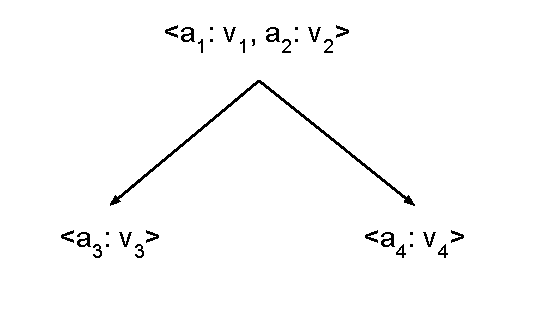
\epsfig{file=PatternExample.pdf}
\caption{An example of transaction, made of three records.}
\label{fig:transaction}
\end{figure}

Let us define a pattern.
\begin{definition}
A pattern is a set of ordered attributes and values belonging to possibly different records in the same transaction. In other words, a pattern is any ordered subset of $\bigcup\limits_{i=1}^{n} \bigcup\limits_{j=1}^{m} \boldsymbol{r_i}<a_j \colon v_j>$, where the ordering is given by the hierarchy of the transaction. For example, in Figure~\ref{fig:transaction} some possible example of pattern are $\{a_1 \colon v_1, a_3 \colon v_3\}$ or $\{a_2 \colon v_2, a_3 \colon v_3\}$, but not $\{a_4 \colon v_4, a_1 \colon v_1\}$, beacuse the latter breakes the hierarchic order.

By definition, since a transaction is structured as a tree, also a pattern is a tree. This means that a pattern must respect the constraints given by the nature of the data structure: each node has at most one parent node, and there are no loops inside the tree, which means that the edges of the tree are meant to be directed from the parent towards the child node.
\end{definition}

Given a set of transactions, the goal is to identify patterns of attributes that are frequent, which means transaction that appear at least a given number of time $f$.

\section{Algorithms}
\label{sec:alg}
The procedure to mine the frequent patterns inside the transactions follows these steps: first of all, the input file is scanned and organized into some data structures; secondly, each transaction is submitted to the frequent itemsets algorithm; thridly, each frequent itemset is analyzed in each transaction, searching if the itemset appears in some ways inside the transaction; finally, the found pattern are counted, and those above the given threshold $f$ are kept and displayed as frequent.

In this section the various parts are described in details.

\subsection{Input parsing and data organization}
As said in Section~\ref{sec:assumptions}, the expected input is composed by a matrix $M \in \Sigma^{n \times d}$, where $\Sigma$ is the dictionary from which the values of the attributes belong to -- it can be a finite subset of $\mathbb{N}$, or a set of strings -- $n$ is the number of records, and $d$ the number of attributes per record. In addition to that, a vector of strings $\boldsymbol{a}$ is needed, containing the names of the attributes. Of course at least three attributes -- \texttt{rid}, \texttt{tid}, \texttt{parent} -- must be part of $\boldsymbol{a}$. Furthermore, an integer threshold $f$ is needed, to decide how many times a frequent pattern has to appear at least.

At the beginning, $M$ is scanned by its rows, and each record (a single row $i$ of the matrix) is saved into a dictionary: the key of a record is its \texttt{rid}, and the content is a set of pairs $<k_j \colon v_j>$, where $k_j = \boldsymbol{a}_j$ and $v_j = M[i,j]$. In this way, given the \texttt{rid}, it is very easy and fast to retrieve the entire record. The dictionary is called $records$. The algorithm to populate this dictionary is trivial, and for this reason is omitted from the report. It is assumed that a dictionary data structure, with a method to add an object giving its key -- $add(key, value)$ -- and a method to search by key and get the relative stored object -- $lookup(key)$ -- exists.

After that, the attributes of the records are analyzed, to reconstruct the transactions. To do so, a data structure -- called Tree --- is used: it is a simple tree made by nodes, where a node can have an arbitrary number of children. This data structure is defined in Table~\ref{tab:tree}. As can be seen, this data structure is needed to keep track of the structure and the hierarchy between nodes belonging to the same transaction. A node having the parent attribute set to the \texttt{null} type -- $\bot$ -- is a root of a transaction.

\begin{table}[H]
\centering
\begin{tabular}{|ll|} \hline
\textbf{Tree} & \\ \hline
\textbf{parent} & Tree \\ \hline
\textbf{children} & Tree[] \\ \hline
\textbf{rid} & string \\ \hline
\textbf{fields} & string[] \\ \hline
\textbf{calls} & int \\ \hline
\textbf{childPatterns} & PNode[][] \\
\hline\end{tabular}
\caption{Tree object definition. The \emph{calls} and \emph{childPatterns} fields are auxiliary variables used for the pattern discovery.}
\label{tab:tree}
\end{table}

To build the transaction, two scans of the dictionary $records$ are needed: the first one to create a node for each record, the second one to assign the degrees of kinship between nodes. In particular, during the second iteration, every node is checked to see if its parent has a value, or it is set to $\bot$: in the first case, it means that the node has a parent, and so its parent is set, and in its parent the node is added as a child; in the second case, it means that the node is a root of a transaction, and so the node is added to a dictionary of treees $roots$. This process is described in the Algorithm~\ref{build_trees}, which returns the dictionary of trees containing the root node of each transaction.

\begin{algorithm}
\caption{Construct the transactions from the dictionary of records $records$.}
\label{build_trees}
\begin{algorithmic}[1]
\Function{generateTrees}{Dictionary $records$}
\State $roots \gets new Dictionary()$
\State $nodes \gets new Dictionary()$
\For{$rid \in records$}
	\State $node \gets new Tree()$ 
	\State $node_{rid} \gets rid$
	\State $nodes.add(rid, node)$
\EndFor
\For{$rid \in records$}
	\State $parent \gets records.lookup(rid)_{parent}$
	\If{$parent = \bot$}
		\State $roots.add(rid, nodes.lookup(rid))$
	\Else
		\State $child \gets records.lookup(rid)$
		\State $parent_{children} \gets parent_{children} \cup \{child\}$
		\State $child_{parent} \gets parent$
	\EndIf
\EndFor
\Return $roots$
\EndFunction
\end{algorithmic}
\end{algorithm}

\subsection{Frequent itemsets in transactions}
Once the input is parsed and the tree structures are built, it is time to apply the frequent itemsets mining algorithm, to search for tuples of attributes that will be the starting point of the frequent pattern mining. As explained in Section~\ref{sec:general}, this approach allows to optimize the number of patterns to search inside the transaction: instead of trying all the possible combinations of attributes, a frequent itemset mining is applied to filter some combinations that for sure would not give any frequent pattern.

The frequent itemset mining algorithm is well known, and it is widely described in \cite{agrawal1994fast}. For this description, it is assumed to have a function $frequentItemsets(String[][]\, item\-sets, float\, sup\-port)$ that takes a list of list of strings, and a floating point number representing the minimum support needed to consider an itemset as frequent. The support of an itemset is the fraction of lists that contains the itemset, over all the lists. This function returns a set if tuples, where each tuple contains an arbitrary number of attributes.

To transform a transaction -- whose structure is a tree -- to a list of strings, the function $flattered(Tree \, t)$ is used. This function has to be able to flatten the tree structure, but also to distinguish between attributes with the same name but with different values. To do so, the name and the value of each attribute of each record are concatenated together, putting in between a special string " = ". For example, if the record $r_1$ has the attribute $<a \colon 1>$ and the record $r_2$ the attribute $<a \colon 2>$, the string version of their attribute is, respectively, "a = 1" and "a = 2". Let us define formaly such function. An important osservation is that the frequent itemsets algorithm works with sets of attributes, so the order with which a transaction is traversed to create its flattened version is indifferent. The procedure is described in Algortihm~\ref{flatten}, which is a wrapper function for the Algorithm~\ref{flattenrec}.

\begin{algorithm}
\caption{Create the flattened version of a transaction.}
\label{flatten}
\begin{algorithmic}[1]
\Function{flatten}{Tree $t$, Dictionary $records$}
\State $itemsets \gets new String[]$
\State $flattenRec(t, records, itemsets)$ \\
\Return $itemsets$
\EndFunction
\end{algorithmic}
\end{algorithm}

\begin{algorithm}
\caption{Recursive function to create the flattened version of a transaction.}
\label{flattenrec}
\begin{algorithmic}[1]
\Function{flattenRec}{Tree $t$, Dictionary $records$, String[] $itemsets$}
\State $record \gets records.lookup(t_{rid})$
\For{$tuple \in record$}
	\State $s \gets tuple_{key} \oplus \text{" = "} \oplus tuple_{value}$
	\State $itemsets \gets itemsets \cup \{s\}$
\EndFor
\For{$child \in t_{children}$}
	\State $flattenRec(child, records, itemsets)$
\EndFor
\EndFunction
\end{algorithmic}
\end{algorithm}

Finally, all the transaction are flattened, and the resulting matrix of strings -- where on the rows there are the various transactions, and on the columns the concatenated attributes -- is given as input to the frequent itemsets algorithm. This can be seen in Algorithm~\ref{freqitemset}. The support value used for the frequent itemsets mining is equal to 0.2.

\begin{algorithm}
\caption{Flat the transaction and compute the frequent itemsets.}
\label{freqitemset}
\begin{algorithmic}[1]
\Function{getFrequentItemsets}{Tree[] $transactions$, Dictionary $records$, float $support$}
\State $globalItemsets \gets new String[][]$
\For{$t \in transactions$}
	\State $flat \gets flatten(t, records)$
	\State $globalItemsets \gets globalItemsets \cup \{flat\}$
\EndFor
\Return $frequentItemsets(globalItemsets, support)$
\EndFunction
\end{algorithmic}
\end{algorithm}

The frequent itemsets functions returns a list of lists of attributes. Each of these lists contain a set of attributes which appears frequently among the transactions. We do not really care about which attribute appears in which set, but we do care about the attributes themselves, because in order to be in any of these sets they have to appear a significant amount of times. The list of lists of attributes is transformed in a set of attributes so that each attribute appears only once. Algorithm ... uses this list to filter frequent attributes in the transactions. To do so, it iterates through every node of every transaction and substitutes the attributes list of the node with the intersection between the latter and the frequent attributes set. The result is a set containing attributes which were in previous attribute list and were also identified as frequent by the frequent itemsets algorithm. The final result of this operation are transactions containing only attributes which appear at least a fixed amount of times among all the transactions.

\subsection{Frequent pattern mining}
\label{sec:patternmining}

The pattern mining process consists in extracting all possible patterns from each transaction and group all of them into one list. At the end of this process, each transaction will have a list containing all possible patterns which are contained in it. In order to store and represent a pattern, a new data structure is defined, called PatternNode -- or PNode for short.

\begin{table}[H]
\centering
\begin{tabular}{|ll|} \hline
\textbf{PNode} & \\ \hline
\textbf{parent} & PNode \\ \hline
\textbf{children} & PNode[] \\ \hline
\textbf{fields} & string[] \\
\hline\end{tabular}
\caption{Pattern node definition.}
\label{tab:tree}
\end{table}

This structure is needed because patterns should only encode their structure and the attributes they contain, they do not need all the other attributes the data structure Tree has. Furthermore, this structure has also some unique methods -- which are described later -- that the Tree structure does not need, and vice versa. Like the Tree structure, PNode has also a \emph{parent} attribute and a \emph{child} attribute, which are used to encode the structure of the pattern which needs to be represented. The \emph{fields} attribute may or may not be empty as patterns may contain nodes which have no fixed attributes and only encode a structural pattern.

The algorithm which computes the pattern uses a recursive bottom up approach starting from each leaf of the transaction and working its way up the tree, while slowly generating all possible nodes and attributes combinations. The algorithm itself takes as input 3 parameters: a PNode representing the current node to be visited which is called $current\-Node$, a list containing all nodes in the transaction called $transaction\-Nodes$, a global list containing all patterns computed up to this point -- called $global\-Patterns$ -- and a list of PNodes containing any pattern to be expanded to the current node, coming from a child, which is called $patterns\-To\-Expand$.

Since the algorithm is very complex, let us start by describing the simplest case: a leaf with no attributes. Initially, the algorithm is called on each leaf of a given transaction. A call to a leaf has the $currentNode$ parameter set to the leaf, the $globalPatterns$ parameter set to a global list defined at a higher level so that it is shared between all the calls of the algorithm for a given transaction, and the $patternsToExpand$ parameter set to an empty list. The only possible pattern which can be generated by the leaf is indeed the empty leaf itself. An empty PNode is generated and appended to the $patternsToExpand$ parameter. Since a single empty PNode cannot be considered a pattern, it is not added to the $globalPatterns$ parameter. Next, the parent is computed by looking for it into the $transactionNodes$ list. If the parent is found, the algorithm is called recursively on the parent with $globalPatterns$ and the new $patternsToExpand$ parameters set. If no parent is found, then the algorithm reached the root and the computation stops as all patterns have been found.

A still simple but more interesting case is when the leaf is not empty and actually contains one or more attributes: differently from the previous case, a PNode for each possible combination of the attributes of $currentNode$ is generated and appended to $patternsToExpand$, together with the empty PNode.  To give an example, let us consider the record $r_1$, having one attribute $<a \colon 2>$ and the record $r_2$ having attributes $<a \colon 4, b \colon 5>$. For record $r_1$ two new PNodes are generated and appended to the $patternsToExpand$ list, one having no attributes and the other one having $<a \colon 2>$. For record $r_2$ four new PNodes are generated and appended to the $patternsToExpand$, one having no attributes, one having $<a \colon 4>$, one having $<b \colon 5>$ and one having $<a \colon 4, b \colon 5>$. Notice that the latter PNode can actually be considered as a horizontal pattern as it has more than one attribute, thus it is appended to the $globalPatterns$ list. 

The two cases that were just described are the simplest cases possible, and they can only happen when the function is computed on leaves. When the function is called on a non-leaf node, all the patterns coming from the children of the node are considered as they should all be expanded by the current node. Let us suppose, in this case, that there is a hierarchical relationship between $r_1$ and $r_2$ from the previous example, where $r_1$ is the parent of $r_2$. Once $r_2$ is computed, appending the four generated PNodes to the $patternsToExpand$ list, the function recursively calls itself with $r_1$ as $currentNode$. The function called on $r_1$ has to combine the patterns coming from its children -- contained in $patternsToExpand$ -- with the two possible PNodes that it generates. In this example, the total patterns generated in $r_1$ and appended to the $patternsToExpand$ list are 10: 4 are the patterns coming from $r2$ combined with the empty PNode generated in $r_1$, 4 more are the patterns coming from $r_2$ combined with the PNode containing $<a \colon 2>$ and the last two are the empty PNode and the latter PNode themselves. The 8 patterns generated by combining the child PNodes with the parent PNodes are all going to be appended to the $globalPatterns$ list, as 6 of them are vertical patterns and 2 are both horizontal and vertical. Notice that if $r_1$ were to have more than one attribute, the PNodes to combine with the child patterns would have been much more.

\begin{algorithm}
\caption{Pattern mining function.}
\label{pattern_mining}
\begin{algorithmic}[1]
\Function{PatternMining}{Tree $currentNode$, Tree[] $transactionNodes$, PNode[] $globalPatterns$, PNode[] $patternsToExpand$}
\State $childCount \gets |currentNode_{children}|$
\If{$|patternsToExpand| > 0$}
    \State $currentNode_{childPatterns} \gets currentNode_{childPatterns} \cup patternsToExpand$
\EndIf
\State $currentNode_{calls} = currentNode_{calls} + 1$
\If{$currentNode_{calls} >= childCount$}
    \State $fieldCount \gets |currentNode_{fields}|$
    \State $newPatterns \gets []$
    \State $newPNodes \gets []$
    \If{$fieldCount > 0$}
        \For{$i \gets 0 \text{ to } fieldCount$}
            \State $fieldsCombinations \gets combinations(currentNode_{fields}, i + 1)$
            \For{$combination \in fieldsCombinations$}
                \State $newNode \gets new PNode()$
                \State $newNode_{fields} \gets combination$
                \State $newNodes \gets newNodes \cup newNode$
                \State $newPatterns \gets newPatterns \cup newNode$
            \EndFor
        \EndFor
    \EndIf
    \State $emptyPNode \gets new PNode()$
    \State $newNodes \gets newNodes \cup emptyPNode$
    \State $newPatterns \gets newPatterns \cup emptyPNode$
    \For{$i \gets 0 \text{ to } childCount$}
        \State $childCombinations \gets combinations(currentNode_{children}, i + 1)$
        \For{$childCombination \in childCombinations$}
            \State $lastChildIndex \gets |childCombination| - 1$
            \State $childCombinatorIndex \gets []$
            \State $childCombinatorSize \gets []$
            \For{$k \gets 0 \text{ to } lastChildIndex + 1$}
                \State $childCombinatorIndex[k] \gets 0$
                \State $childCombinatorSize[k] \gets |childCombination[k]|$
                \While{$childCombinatorIndex[0] < childCombinatorSize[0]$}
                    \State $patternsToCombine \gets []$
                    \For{$j \gets 0 \text{ to } lastChildIndex + 1$}
                        \State $patternsToCombine[j] \gets childCombination[j][childCombinatorIndex[j]]$
                    \EndFor
                    \For{$node \in newNodes$}
                        \For{$z \gets 0 \text{ to } lastChildIndex + 1$}
                            \State $toAppend \gets toCombine[z]$
                            \State $node_{children} \gets node_{children} \cup toAppend$
                            \State $toAppend_{parent} \gets node$
                        \EndFor
                        \State $newPatterns \gets newPatterns \cup node$
                    \EndFor
                    \State $childCombinatorIndex[lastChildIndex] \gets childCombinatorIndex[lastChildIndex] + 1$
                    \For{$z \gets lastChildIndex \text{ to } 0$}
                        \If{$childCombinatorSize[z] - childCombinatorIndex[z] = 0$}
                            \State $childCombinatorIndex[z] \gets 0$
                            \State $childCombinatorIndex[z - 1] \gets childCombinatorIndex[z - 1] + 1$
                        \EndIf
                    \EndFor
                \EndWhile
            \EndFor
        \EndFor
    \EndFor
    \For{$pattern \in newPatterns$}
        \If{$|pattern_{children}| > 0 OR |pattern_{fields}| > 1$}
            \State $globalPatterns \gets globalPatterns \cup pattern$
        \EndIf
    \EndFor
    \State $parent \gets \bot$
    \For{$node \in transactionNodes$}
        \If{$node_{rid} = currentNode_{parent}$}
            \State $parent \gets node$
        \EndIf
    \EndFor
    \If{$parent != \bot$}
        \State $PatternMining(parent, transactionNodes, globalPatterns, newPatterns)$
    \EndIf
\EndIf
\EndFunction
\end{algorithmic}
\end{algorithm}

The last and most complex case happens when the function is called with a non-leaf node as $currentNode$ having more than one children. This case is particularly complex because a pattern may involve 2 children starting from the $currentNode$, thus all the combinations of all the patterns from all the children must be considered and combined with the PNodes generated in the $currentNode$. As an example, consider the previously mentioned $r_1$ and $r_2$ having the same hierarchical structure ($r_1$ parent of $r_2$) and let us introduce another record $r_3$, child of $r1$, having as attributes $<a \colon 1, b \colon 6>$. Firstly, the algorithm needs to ensure that before computing the patterns of $r_1$, all of its children have already computed theirs. In order to do this, the Tree object has an integer attribute called \emph{calls}, which acts as a synchronization method. Each time a child completes its pattern generation and recursively calls the mining function with its parent as $currentNode$, the \emph{calls} attribute of the parent is incremented by 1. If the value of calls on the parent node is equal to the number of its children, it means that all the children have generated their patterns and the parent can start computing its own. This means that if $r_2$ were to generate its 4 PNodes and call the function on $r_1$, the generation process would not start for $r_1$ as $r_3$ still has to compute its patterns. Once $r_3$ is also finished, it will recursively call the function on $r_1$ which will now have the value of its \emph{calls} attribute equating the number of its children. Furthermore, each time a child calls the function on its parent, and not all of its children are done computing, the $patternsToExpand$ parameter coming from the child needs to be stored or otherwise it would be lost. To allow parent nodes to store children patterns, each Tree object also has a \emph{childPatterns} attribute. Each element of this array represents a list of pattern of a child. Notice that even if a node were to have only one child, the \emph{calls} attribute on the parent is incremented anyway, and the child patterns are still stored in \emph{childPatterns} array. Let us now suppose that both $r_2$ and $r_3$ are done computing their patterns and have already passed them to $r_1$. $r_1$ firstly generates its two PNodes, one with $<a \colon 2>$ and one with no attributes. Secondly, the combination of children patterns are computed, and in this case a possible pattern may involve only patterns coming from $r_2$, or only patterns coming from $r_3$, or patterns coming from both of them. For the first two cases the algorithm is just going to combine each pattern of a child with its own two PNodes. For the third case the algorithm is going to combine each combination of patterns coming from the children with its own PNodes. By combination of the patterns of the children, is meant each pattern in $r_2$ coupled with each pattern in $r_3$. The total number of patterns generated by $r_1$ is 50: 8 from the combinations of $r_2$ patterns with $r_1$ PNodes, 8 from the combinations of $r_3$ patterns with $r_1$ PNodes, 32 from the combination of $r_2$ and $r_3$ patterns with $r_1$ PNodes and 2 from $r_1$ PNodes themselves. All 50 patterns are going to be appended to the $patternsToExpand$ list and passed to the parent of $r_1$, if it exists, while 48 of these patterns are going to be appended to the $globalPatterns$ list.

To summarize, the mining algorithm is called on each leaf of a transaction and is going to recursively combine the patterns generated in the child nodes with the PNodes generated in the parents. This method, while extremely computationally expensive, allows to find every possible pattern that there could be in the transaction.

There is a variation to the mining algorithm where for each $currentNode$ is checked whether it has some attributes or not. In case it does not we discard all the patterns passed from the child in the $patternsToExpand$ list, and the function is called on the parent. Furthermore, when the PNodes of a given $currentNode$ are generated, the \emph{empty} PNode is not considered. With this small change is possible to drastically reduce computational complexity at the cost of only finding contiguous patterns, meaning patterns composed only by nodes having at least one fixed attribute in the pattern.

The pattern mining algorithm is shown in Algorithm \ref{pattern_mining}. It is assumed that a function $combinations$ exists taking as input a list $L$ and an integer $len$ and returning a matrix containing all the possible $len$ long combinations of the elements in $L$.

\subsubsection{Computational Complexity}
In this section is shown an example of how big of an impact the implementation has on the base complexity of the problem. Consider the transaction represented in Figure \ref{fig:transactionFullComplexity}.

\begin{figure}[h!]
\centering
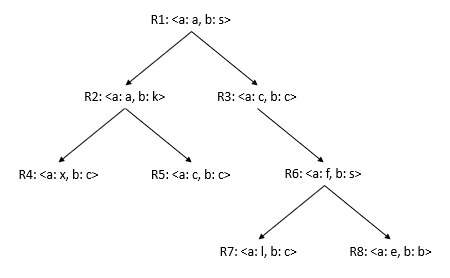
\includegraphics[width=0.5\textwidth]{FullTransactionExample.jpg}
\caption{Example of transaction.}
\label{fig:transactionFullComplexity}
\end{figure}

Let us simulate the pattern mining process on the transaction without performing any kind of attribute filtering, while keeping track of the patterns found. Starting from the leaves, the number of patterns generated in $R7$ and in $R8$ is 4 each. Only the PNodes with both attributes present are inserted into the global pattern list, thus the pattern count is equal to 2. $R6$ also generates 4 PNodes, as it has 2 attributes; however, it also needs to combine its own PNodes with the children patterns. The combinations are: patterns from $R7$ with PNodes of $R6$, patterns from $R8$ with PNodes of $R6$ and patterns from both $R7$ and $R8$ with PNodes of $R6$. The total of patterns generated by performing these combinations is computed as 4 * 4 + 4 * 4 + 4 * 4 * 4 = 96. To this total we also need to sum the 4 PNodes of $R6$ bringing the count up to 100. Of all these patterns, only 97 are going to be appended to the global pattern list, as only 1 of the PNodes generated in $R6$ can be considered a pattern. The global pattern list amounts to 99 patterns now. $R3$ has to combine its 4 PNodes with the patterns generated in $R6$ for a total of 4 * 100 = 400 patterns plus 4 PNodes from $R3$. Of these 404 patterns, 401 are going to be added to the global pattern list, bringing the total up to 500. Similarly to $R6$, $R2$ is also going to generate 100 patterns and 99 of them are added to the total, which now amounts to 599. $R1$ can now generate its own patterns by combining its 4 PNodes with the patterns generated by its children. The total of patterns generated by $P1$ is computed as 100 * 4 + 404 * 4 + 100 * 404 * 4 = 163616. To this total we sum the 4 PNodes of $R1$ and add 163617 patterns to the global patterns list, bringing the final patterns count to 164216 patterns.

Let us now simulate the pattern mining process on the transaction by performing attribute filtering. By filtering the attributes and keeping only the ones which are frequent enough among all the transactions we end up with the transaction shown in Figure \ref{fig:transactionTrimmedComplexity}.

\begin{figure}[h!]
\centering
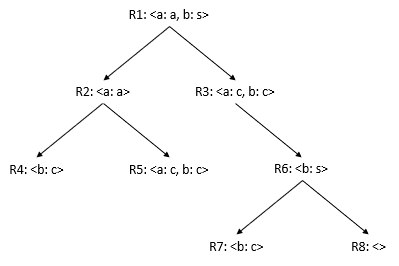
\includegraphics[width=0.5\textwidth]{TrimmedTransactionExample.jpg}
\caption{Example of filtered transaction.}
\label{fig:transactionTrimmedComplexity}
\end{figure}

Starting from the leaves, the number of patterns generated in $R7$ and $R8$ are 2 and 1 respectively. None of these 3 patterns is added to the global patterns list as none of them is eligible. $R6$ needs to combine its 2 PNodes with the children patterns. The combinations are computed as 2 * 2 + 2 * 1 + 2 * 2 * 1 = 9. By adding $R6$ PNodes the total generated patterns are 11. We add 9 of these patterns to the global pattern list as $R6$ PNodes are not eligible. $R3$ combines its 4 PNodes with the 11 patterns coming from $R6$ for a total of 44 patterns plus 4 PNodes. Of these 48 patterns, 45 are going to be added to the global pattern list bringing the total pattern count to 54. $R4$ and $R5$ are going to generate 2 and 4 patterns respectively and $R5$ is going to add one of its 4 patterns to the global patterns list bringing it up to 55 patterns. $R2$ is going to combine the patterns coming from its children with its 2 PNodes. The combinations are computed as 2 * 2 + 4 * 2 + 2 * 4 * 2 = 28. Adding 2 PNodes from $R2$ the patterns generated add up to 30. 28 of these are going to be added to the global pattern list which now equals to 83. Lastly, $R1$ combines its 4 PNodes with the patterns coming from $R2$ and $R3$. The combinations are going to be computed as 30 * 4 + 48 * 4 + 30 * 48 * 4 = 6072. To these patterns we add 4 PNodes from $R1$ bringing the total up to 6076 patterns, of which, 6073 are going to be added to the global pattern list which now amounts to 6128 patterns.

Both of the pattern sets generated in the two simulations contain the frequent patterns that are looked for. The patterns found in the first simulation are made up by both non frequent attributes, which cannot be part of a frequent pattern, and frequent attributes. While being only 0.037\% of the patterns found in the first simulation, the patterns generated by the second simulation are made up exclusively by frequent attributes and the frequent patterns are guaranteed to be among them. It is pretty obvious that the complexity of the problem depends on many variables and can scale up a lot by just adding a node or an attribute. Even by removing a single attribute the problem becomes much smaller. Our implementation allows to remove as many attributes as possible in order to decrease the number of patterns to consider.

\subsection{Pattern count and selection}
Once all the candidate patterns are generated, it is time to group those that are equal, and to count them. To do so, a dictionary is used, with keys the candidate patterns, and values the counter of the relative pattern. Because of this data structure, it is possible to count all the candidate patterns in linear time with respect to the number of candidates: in fact, it is necessary just to visit each pattern once, verify if it is already in the dictionary -- in case it is, is sufficient to increment the counter, otherwise a new object is inserted in the dictionary, with its count equals to 1.

To operate with a dictionary, it is necessary that the objects used as keys define an equals function and a hash function: the two functions are very similar, and they are both take count of the attributes of the transaction, but also the length and the structure of it. They are defined recursively, starting from the roots of the trees: two patterns are equals if the root nodes have the same attributes and if the set of children of one root is equals to the set of children of the other. The same can be said for the hash function: two transactions have the same hash value if the roots are equals, and if the children of one are equals to the children of the other. Two leaves are equals -- have the same hash value -- if they have the same attributes. Of course the ordering of the attributes and children has no importance in this scenario, the only important thing is that two nodes that are equal must have the same content. For this reason, mathematical sets are used with attributes and children. Two sets $S_1$ and $S_2$ are equals if $S_1 \subseteq S_2 \land S_2 \subseteq S_1$. The hash function of a set is the hash of its content, in this case strings or other PatternTree, while the hash of a tuple is the concatenation of the hash of its elements. The equal function between two PatternTree is shown in Algorithm~\ref{equals}, while the hash function of a PatternTree is defined in Algorithm~\ref{hash}. Both the function have a complexity that is linear to the number of nodes that compose a pattern, since every node is visited to compute the two functions.

\begin{algorithm}
\caption{Comparison between two PatternTree.}
\label{equals}
\begin{algorithmic}[1]
\Function{equals}{PatternTree $p_1$, PatternTree $p_2$}
\State $attributes_1 \gets \{i : i \in p_1.fields\}$
\State $attributes_2 \gets \{i : i \in p_2.fields\}$
\State $children_1 \gets \{c : c \in p_1.children\}$
\State $children_2 \gets \{c : c \in p_2.children\}$
\State $length_1 \gets 1 + |children_1|$
\State $length_2 \gets 1 + |children_2|$ \\
\Return $attributes_1 = attributes_2 \land children_1 = children_2 \land length_1 = length_2$
\EndFunction
\end{algorithmic}
\end{algorithm}

\begin{algorithm}
\caption{Hash function of a PatternTree.}
\label{hash}
\begin{algorithmic}[1]
\Function{hash}{PatternTree $p$}
\State $attributes \gets \{i : i \in p.fields\}$
\State $children \gets \{c : c \in p.children\}$
\State $length \gets 1 + |children|$ \\
\Return $hash(attributes, children, length)$
\EndFunction
\end{algorithmic}
\end{algorithm}

At this point is possible to proceed to count how many times a pattern appears among the all transaction. As said, to do so a new dictionary -- called $filter$ -- is created, and iterating over all the found candidate patterns, it is just necessary to check whether the current pattern is already in the dictionary or not.

Once all the patterns are counted, two other operations are performed: sorting and filtering. Not all the patterns have the same relevance: the more frequent a pattern is, the more important, but also the larger it is, the more important. To decide this relation of \emph{importance} between patterns, a function is defined, that takes count of both the length and the frequency of the pattern. The length of a pattern is the number of nodes it contains, while the frequency is how many time it appears among the transactions. The \emph{importance} function is defined as follows:
\begin{gather}
\begin{split}
importance & \colon PatternNode \to \mathbb{N} \\
importance & \colon node \mapsto node_{length} \times node_{frequency}
\end{split}
\end{gather}

As regards the filtering, it is very simple: all the patterns that appear less than a given number of times $f$, they are discarded.

The whole procedure is defined in Algorithm~\ref{counting}: the patterns are counted, filtered and then sorted. Finally, the sorted list is returned, assuming that $sortByImportance$ sorts the dictionary using the \emph{importance} function, and returns a list of patterns.

\begin{algorithm}
\caption{Count, filter and sort the patterns.}
\label{counting}
\begin{algorithmic}[1]
\Function{CountSortFilter}{PatternNode[] $candi\-da\-tes$, Integer $f$}
\State $filter \gets new Dictionaty()$
\For{$pattern \in candidates$}
	\State $stored \gets filter.lookup(pattern)$
	\If{$stored = \bot$}
		\State $filter.add(pattern, 1)$
	\Else
		\State $stored \gets stored + 1$
	\EndIf
\EndFor
\For{$pattern \in filter$}
	\If{$filter.lookup(pattern) < f$}
		\State $filter.remove(pattern)$
	\EndIf
\EndFor
\Return $sortByImportance(pattern)$
\EndFunction
\end{algorithmic}
\end{algorithm}

To sum up, the whole procedure to mine the frequent subtree in the transaction is the following: the input matrix is read and organized in a dictionary, with one entry for every record; from the records, the tree-structured transaction are reconstructed with the Algorithm~\ref{build_trees}; each record is flattened into a list of string with Algorithm~\ref{flatten}, and the resulting list of strings is used in Algorithm~\ref{freqitemset}; starting from the frequent combinations of attributes, the candidate patterns are generated using Algorithm~\ref{pattern_mining}, and finally they are counted, sorted and filtered by the Algorithm~\ref{counting}.

\section{Implementation}
The steps and algorithms described in Section~\ref{sec:alg} are implemented in a program, that takes as input a \texttt{csv} file, and integer $f$ and writes its output in a \texttt{txt} file. In particular, the input file is the translation of the matrix $M$ described in the assumptions -- Section~\ref{sec:assumptions} -- and it is expected to have $n + 1$ lines, where the first line contains the list of the names of the attributes of each record, and the following $n$ lines contains the attribute values of each record. The integer $f$ is the threshold over which a pattern is considered frequent -- it is called $thr$ in the program -- and in the output file are printed the frequent patterns ordered by their importance. For each frequent pattern, its frequency, its length, its importance value and the whole pattern are included in the output file. 

The patterns are printed like trees, where two nodes on the same identation level are siblings. Every node with identation level $i$ is child of the previous node that has an identation level $i - 1$. Furthermore, in each node are indicated the list of names and values of attributes that compose the pattern: an empty node -- with an empty list of such attributes -- is any possible node, with any possible attribute names and values.

The software is written in Python\footnote{www.python.org}, and it makes use of the Pandas\footnote{pandas.pydata.org} library \cite{mckinney2010data} and the \texttt{mlxtend} library for the frequent itemset mining\footnote{rasbt.github.io/mlxtend}. In particular, the latter library works with an one-hot encoding of the attributes of the nodes, and for this reason Pandas is used, as suggested by the documentation of \texttt{mlxtend}.

The software is developed using an object oriented paradigm, and therefore it is composed by many small components that interact with each other. Each of this component has been tested, with several test cases, to verify its behaviour and its correctness.

\subsection{Use the software}
To use the software, it is mandatory to have a Python interpreter installed, at least with version 3.6, and to install the dependencies -- the libraries needed by the software -- by running the command \texttt{pip install -r requirements.txt}. To launch the software it is necessary to run the command \texttt{python src/main.py <arguments>}, with the following possible argument list:
\begin{itemize}
\item \texttt{-out filename}, to specify the filename on which the output is written. Default is \texttt{output.txt};
\item \texttt{-in filename}, to specify the file from which the input is read. It has to be a \texttt{csv} file. Default is \texttt{input.csv};
\item \texttt{-thr integer}, the minimum number of times a pattern has to appear to be considered frequent. Default is 4;
\end{itemize}
 
\section{Experiments}
The software has been tested and compared with the so called \emph{baseline}, another software that does the same operation with a different approach. In this section the \emph{baseline} is briefly described, and then the results of the experiments are given.

\subsection{The baseline}
As said, the baseline is another software that does the same task of the one described in this report, with which our software is compared. In particular, the baseline uses the same approach described in Section~\ref{sec:patternmining}, but without the attribute filter made with the frequent itemset mining algorithm. 

Algorithmically speaking, the baseline does the following: the input matrix is read and organized in a dictionary, with one entry for every record; from the records, the tree-structured transaction are reconstructed with the Algorithm~\ref{build_trees}; the whole list of transaction is used as input for the candidate pattern mining algorithm -- in this way there are much more combination of attributes that the algorithm has to check, and finally they are counted, sorted and filtered by the Algorithm~\ref{counting}.

In this way, it is possible to demonstrate the validity of the optimization performed filtering the less frequent combination of attributes using the frequent itemset mining algorithm. The next subsection shows the results of the performed experiments.

\subsection{Experiment results}
\label{sec:exp-res}
Analyze this software is very hard, because the final results strongly depend on how the input is structured, and not by the parameters with whom the input was generated. As it is described in this section, there are \emph{smaller} input -- in terms of number of records and transactions -- that takes much more time and resources with respect to \emph{larger} ones. The real magnitude of complexity is given by the cardinality of the set of all the frequent patterns that exist in the input transactions. This number is not related with the number of transactions inside the input, or with the number of patterns generated, but only with the complexity of such patterns: in fact, a complex pattern that involves several nodes gives rise to many sub-patterns, and since the bigger one is frequent, all the smallers are frequent too. Let us give an example: a pattern made of three nodes, each one with two attributes, includes a total number of 63 different frequent patterns. In fact, for each node a pattern with all the attributes, with only one attribute and with no attributes exists -- 4 possibility -- multiplying these combinations with all the 3 nodes -- $4 \times 4 \times 4$ -- and removing the case in which all the nodes are \emph{empty} -- which means that in each node any possible value is accepted, which is not a pattern -- gives 63 combinations. In general, the combinations of a pattern made by $m$ nodes, each one with at most $n$ attributes that belong to the pattern, have an upper buond equals to $2^{n \times m} - 1$. Of course, the more complex a pattern is, the more the problem explodes.

In general, 5 datasets were generated with the generator -- see the big data report for further details about such generator -- and used for the tests: all of them constains two main patterns distributed over 1, 2, 5, 10 and 20 transaction respectively. Three types of tests are performed: one to compare the baseline and our algorithm while mining all the possible patterns, another one mining only patterns without \emph{empty} nodes, and finally a test comparing the outcomes of our algorithm changing the support hyperparameter of the frequent itemset mining. In the next subsections these tests are described in details.

All the test are performed on a machine with a 2GHz Intel Core i7 processor, and 8GB of RAM.

\subsubsection{All pattern test}

\begin{figure}
\centering
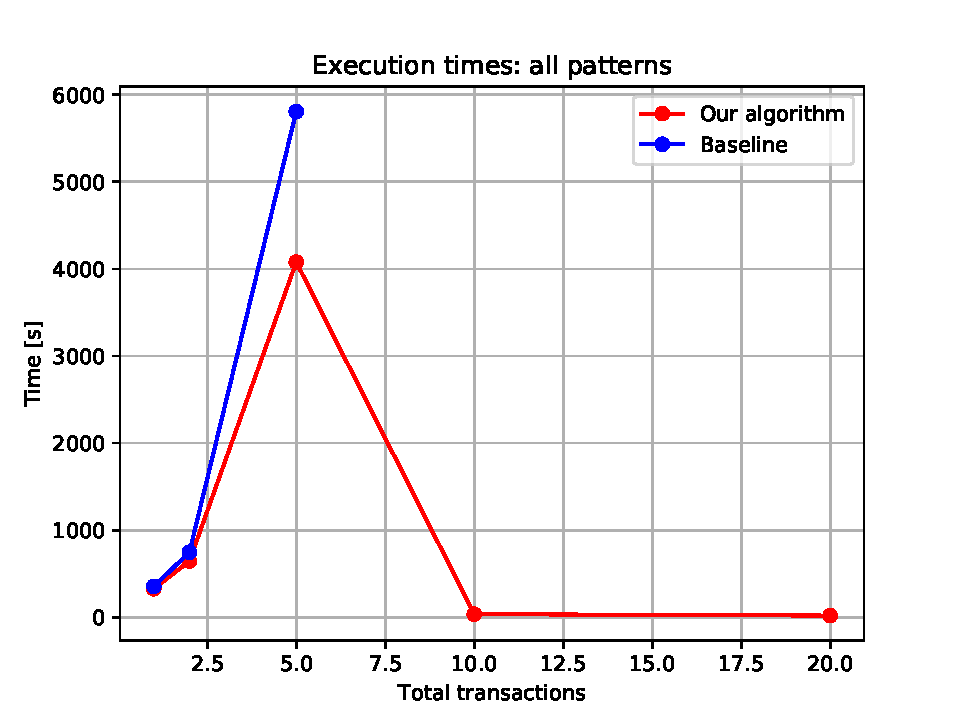
\epsfig{file=test1.pdf, scale=0.5}
\caption{Comparison of the execution times between our solution and the baseline. Since the last two inputs were not testable on the baseline, they are not reported in the graph.}
\label{fig:testone}
\end{figure}

The very first conducted test is about the performance comparison between our algorithm and the baseline. In addition to that, also the cardinality of the resulting sets of frequent pattern is analyzed.

In particular, for each available dataset, both the software are used, timing their executions and saving their outputs. As regards the outputs, they turned out to be always the same: the two sets have always been equals to each other. This means that applying a filter on the attribute values using the frequent itemset mining algorithm with a support value equals to 0.2 did not exclude any valid frequent pattern. Since the two sets are equals, they are not plotted in any way, but their cardinality is now given:
\begin{itemize}
\item the first input, with one transaction, gives rise to 52977 frequent patterns;
\item the second input, with two transactions, gives rise to 49162 frequent patterns;
\item the third input, with five transactions, gives rise to 777174 frequent patterns;
\item the fourth input, with ten transactions, gives rise to 11899 frequent patterns;
\item the fifth input, with twenty transactions, gives rise to 9783 frequent patterns.
\end{itemize}

As regards the times of the exectutions, those of our algorithm have always been definitely lower than those of the baseline. Furthermore, for the fourth and the fifth input, it was not possible to test the baseline, since after several hours of executions, the operative system killed their respective processes. Investigating a bit, the reason was that the processes was taking almost the entirety of the RAM, and also around 40GB of the SSD space. For this reason, the graph in Figure~\ref{fig:testone} shows only a partial curve for the baseline times. 

In both the latter graph and the latter list is possible to observe what is said in Section~\ref{sec:exp-res}: the exectution times depends on the complexity of the patterns, and therefore by how many sub-patterns is possible to find.

\subsubsection{Contiguous pattern test}

\begin{figure}
\centering
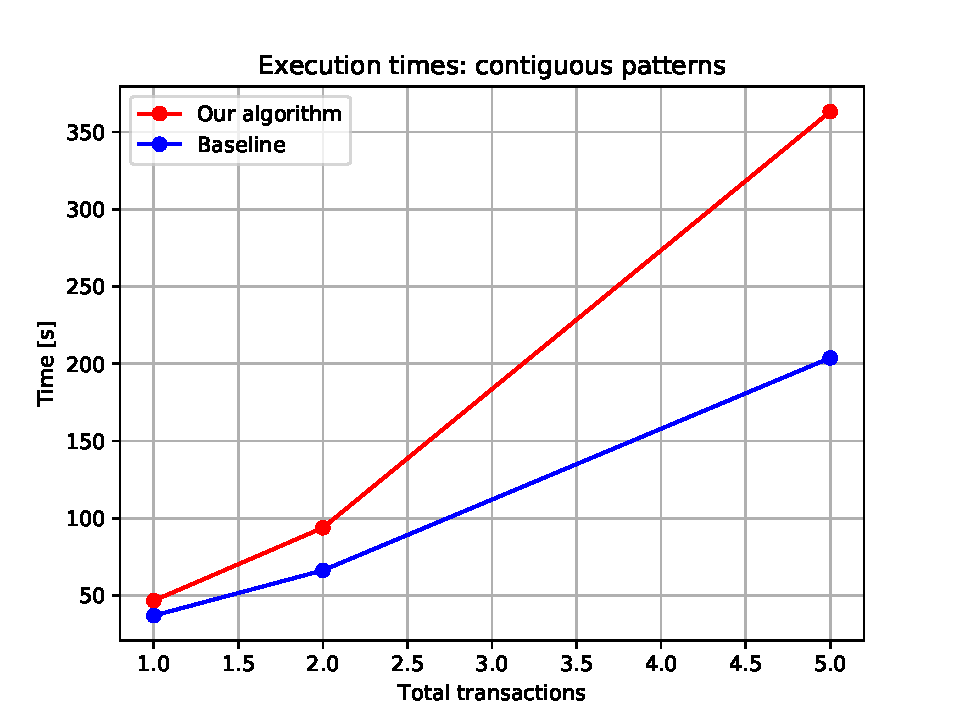
\epsfig{file=test2.pdf, scale=0.5}
\caption{Comparison of the execution times between our solution and the baseline looking for contiguous patterns only. Only the first three cases are plotted, since the last two gave results with a very different magnitude -- too high for the baseline, too low for our algorithm -- and for scaling reasons they are omitted.}
\label{fig:testtwo}
\end{figure}

In the second test only the \emph{contiguous} patterns are searched for, or those patterns where each node that compose them has specific values for the attributes involved in the pattern. In other words, these kinds of patterns are composed by a specific set of attributes spreaded among nodes, and there are no generic nodes that can be composed by any possible attribute.

This test is performed to see how the two solutions perform with an easier task, that lowers the complexity of finding the frequent patterns. Also in this case, both the execution times and the cardinalities of the outcomes are considered. The latter are much smaller than the ones in the first test, as can be seen in the following list:
\begin{itemize}
\item the first input, with one transaction, gives rise to 0 frequent patterns with only contiguous nodes;
\item the second input, with two transactions, gives rise to 5 frequent patterns with only contiguous nodes;
\item the third input, with five transactions, gives rise to 48683 frequent patterns with only contiguous nodes;
\item the fourth input, with ten transactions, gives rise to 16 frequent patterns with only contiguous nodes;
\item the fifth input, with twenty transactions, gives rise to 28 frequent patterns with only contiguous nodes.
\end{itemize}

As regards the exectution times, they are also much smaller than the previous test: in this case also with the fourth and the fifth inputs the baseline program was able to terminate, but with very high execution times: with the fourth, the baseline took around 4 hours, while with the fifth around 6 hours. On the other hand, our solution took less than a second with the last two inputs. To avoid scale problems, the fourth and the fifth cases are omitted from the graph in Figure~\ref{fig:testtwo}, that shows only the first three cases. 

In conclusion, in these tests the performances of the two algorithms can vary a lot: as can be seen in Figure~\ref{fig:testtwo}, with three inputs out of five, the baseline was faster, but in the last two cases our solution was definitely faster.

\subsubsection{Different support values for the frequent itemsets algorithm}

\begin{figure}
\centering
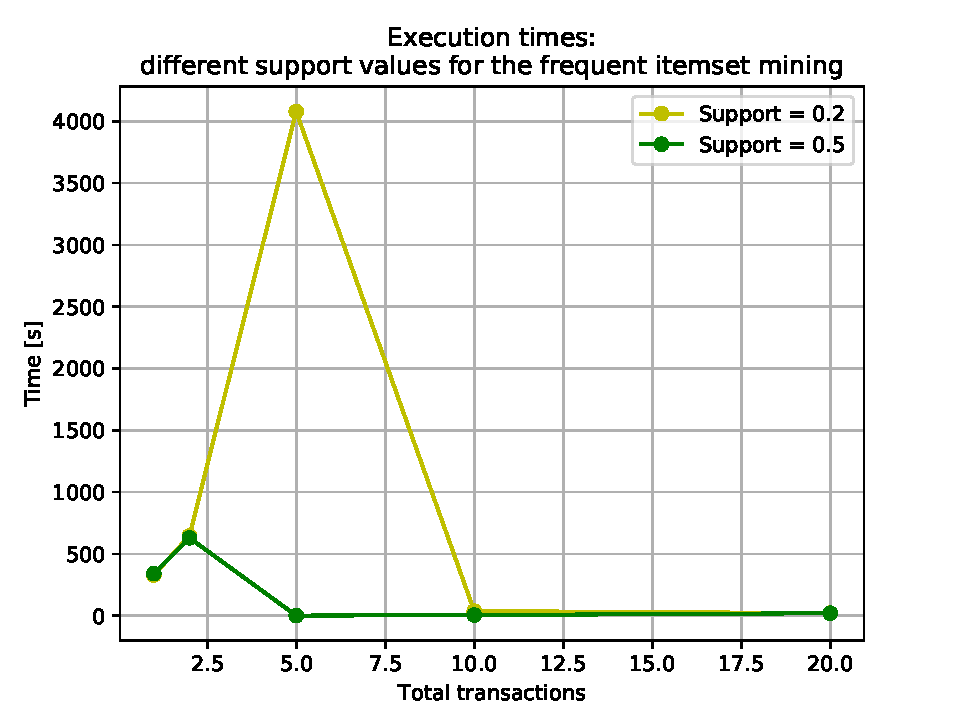
\epsfig{file=test3.pdf, scale=0.5}
\caption{Comparison of the execution times using different values for the support in the frequent itemset mining algorithm.}
\label{fig:test3}
\end{figure}

\begin{figure}
\centering
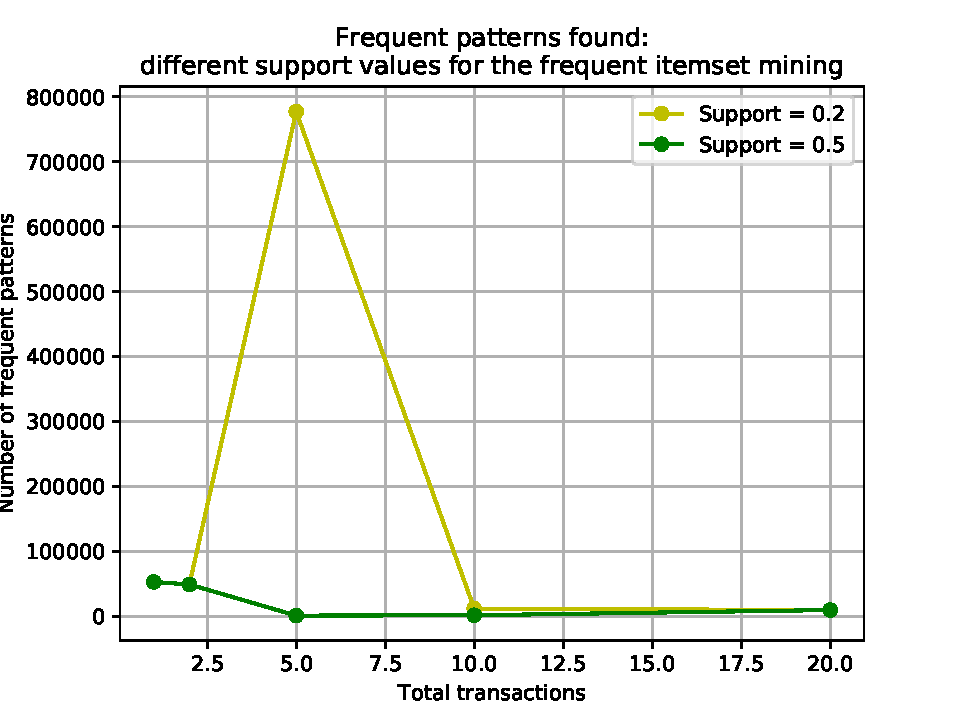
\epsfig{file=test4.pdf, scale=0.5}
\caption{Comparison of the cardinality of the resulting sets of frequent patterns using different values for the support in the frequent itemset mining algorithm.}
\label{fig:test4}
\end{figure}

An important hyperparameter that influences on the behaviour of the algorithm is the support value given to the frequent itemset mining algorithm, which represent the minimum value of the fractions of itemsets that contains a specific item to consider such item as frequent. The higher this value, the more selective the algorithm is. As a consequence, the more the algorithm is selective, the less combinations are tried by our procedure, but also the less candidate patterns are generated. For this reason, two different values for the hyperparameter are tested: 0.2 and 0.5 respectively.

The Figure~\ref{fig:test3} shows the response time differences using the two different values: of course, the higher the parameter, the less combinations are tried, and so the response time is always lower using the higher value. On the other hand, as can be seen in Figure~\ref{fig:test4}, the lower value offers a much more precise output: in fact, the cardinality of the set of the frequent patterns is always greater when the support value is equals to 0.2.

In conclusion, is was decided to reward the precision with respect to the performance, and for this reason the used value of the support for the frequent itemset mining algorithm is equal to 0.2.

\section{Conclusions}
In this paper were described the methods used, the algorithms developed and the results obtained during the implementation of an application for frequent itemsets mining in tree-like sequences of complex objects. It was demonstrated how big the task is in terms of complexity. Our implementation allows to make the problem more approachable by filtering attributes which are guaranteed to not appear in any frequent pattern as they do not appear enough times among all objects in order to be frequent. Our method was also compared with the baseline which tackles the full size problem without any filtering performed on the attributes. The comparisons demonstrated that our method generally allows to make the problem several orders of magnitude smaller. It must be said that in some cases our algorithm would not bring any improvement compared to the baseline, consider transactions composed only by frequent patterns for example. However, in the average instance there will always be at least one attribute which can be safely removed without losing any frequent pattern allowing to make the problem considerably smaller.

%\end{document}  % This is where a 'short' article might terminate
%
% The following two commands are all you need in the
% initial runs of your .tex file to
% produce the bibliography for the citations in your paper.
\bibliographystyle{abbrv}
\bibliography{sigproc}  % sigproc.bib is the name of the Bibliography in this case
\end{document}
